%%%%%%%%%%%%%%%%%%%%%%%%%%%%%%%%%%%%%%%%%%%%%%%%%%%%%%%%%%%%%%%%%%%%%%
%% On jet mass corrections and transversity
%% May 10, 2013
%%%%%%%%%%%%%%%%%%%%%%%%%%%%%%%%%%%%%%%%%%%%%%%%%%%%%%%%%%%%%%%%%%%%%%
\documentclass[preprintnumbers,floatfix,nofootinbib]{revtex4}

\usepackage[tbtags]{amsmath}  % AMS math 
\usepackage{amssymb}          % AMS symbols
\usepackage{bm}               % bold math
\usepackage{graphicx}         % PostScript figures
\usepackage[export]{adjustbox}% to align images
\usepackage{hhline,multirow}  % for nicer tables
\usepackage{dcolumn}          % Align table columns on decimal point
\usepackage{slashed}
\usepackage{datetime}
\usepackage{color}
\usepackage[dvipsnames]{xcolor}

%%%%%% for draft
\newcommand{\todo}[1]{\marginpar{$\bullet$}\textbf{#1}}
\def\AAcom#1{{\bf  \textcolor{Red}{[AA: {#1}]}}}
\def\AAmod#1{{\textcolor{Green}{#1}}}

%%%%%%  Definitions   %%%%%%%%%%%
  
\newcommand{\Pslash}{P \hspace{-0.24cm} / \,}
\newcommand{\kslash}{k \hspace{-0.21cm} / \,}
\newcommand{\lslash}{l \hspace{-0.19cm} / \,}
\newcommand{\nslash}{n \hspace{-0.24cm} / \,}
\newcommand{\vslash}{v \hspace{-0.21cm} / \,}
\newcommand{\Sslash}{S \hspace{-0.22cm} / \,}
\newcommand{\Dslash}{D \hspace{-0.22cm} / \,}
\newcommand{\epsslash}{\varepsilon \hspace{-0.18cm} / \,}
\newcommand{\Tr}{\operatorname*{Tr}\nolimits} % Trace operator
\newcommand{\xbj}{x}                   % Bjorken variable
\newcommand{\de}{d}                    % differential
\newcommand{\ii}{i}                    % imaginary unit

\newcommand{\eg}{{\em e.g.}}
%\newcommand{\mj}{\langle m_j \rangle}
%\newcommand{\mj}{M_q^\text{jet}}
\newcommand{\mj}{M_q}
\newcommand{\mq}{m_q}
\newcommand{\mjs}{\langle m_j^2 \rangle>}

\allowdisplaybreaks[2]

\begin{document}

%%%%%%%%%%%%%%%%%%%%%%%%%%%%%%%%%%%%%%%%%%%%%%%%%%%%%%%%%%%%%%%%%%%%%%
%%%%%%%%%%%%%%%%%%%%%%%   TITLE    %%%%%%%%%%%%%%%%%%%%%%%%%%%%%%%%%%%
%%%%%%%%%%%%%%%%%%%%%%%%%%%%%%%%%%%%%%%%%%%%%%%%%%%%%%%%%%%%%%%%%%%%%%

\preprint{JLAB-THY-16-????}

\title{Accessing the nucleon tensor structure in inclusive deep inelastic scattering} 

\author{Alberto~Accardi$^{a}$, Alessandro~Bacchetta$^{b}$} 
\affiliation{
$^a$Jefferson Lab, Newport News, VA 23606, USA, and
Hampton University, Hampton, VA 23668, USA \\
$^b$Dipartimento di Fisica, Universit\`a degli Studi di Pavia, and INFN,
Sez. di Pavia, 27100 Pavia, Italy
}

\date{\bf \today, \currenttime}

\begin{abstract}

\end{abstract}

%\pacs{ }

%\keywords{ }

\maketitle


%%%%%%%%%%%%%%%%%%%%%%%%%%%%%%%%%%%%%%%%%%%%%%%%%%%%%%%%%%%%%%%%%%%%%%%%%
\section{Introduction}

The tensor charge is a fundamental property of the nucleon, at
present poorly constrained. It has been estimated in lattice
QCD (see, \eg,
\cite{Green:2012ej,Bali:2014nma,Bhattacharya:2015wna,Abdel-Rehim:2015ow}), but
only limited information is available from direct measurements. The
way to extract the tensor charge from experimental measurements requires first
of all the extraction the so-called transversity parton distribution function,
denoted by $h_1^q(x)$~\cite{Radici:2015mwa,Anselmino:2015sxa,Kang:2015msa}. 
The integral of the transversity distribution
corresponds to the contribution of flavor $q$ to the tensor charge.

In this paper, we discuss the possibility of observing the effect of
the transversity parton distribution function (PDF) in totally inclusive Deep Inelastic Scattering.

The transversity distribution is notoriously difficult to access because it is
a chiral-odd function and needs to be combined with a spin-flip mechanism to
appear in a scattering process~\cite{Jaffe:1996zw,Barone:2001sp}. Usually, this spin flip is provided by another
nonperturbative distribution or fragmentation function, implying that
transversity cannot be accessed in inclusive DIS,
but only in more complex processes such as semi-inclusive DIS or Drell-Yan~\cite{Ralston:1979ys,Jaffe:1991kp,Jaffe:1993xb,Collins:1993kk}. 

The only other way to attain spin-flip terms in QED and QCD is taking into
account mass corrections. In fact, it is well known that transversity gives a
contribution to the structure function $g_2$ in inclusive DIS (see, \eg,
\cite{Accardi:2009au} and references therein), and in
particular to the violation of the so-called Wandzura--Wilczek relation for
$g_2$~\cite{Wandzura:1977qf}. However, this contribution is proportional to the current quark mass
and can be expected to be very small.

We revisit the standard analysis of inclusive DIS taking into account the fact
that on-shell quarks cannot be present in the final state, but they rather
decay into hadrons (ideally, forming jets of hadrons). This is sufficient to modify the structure of the DIS
cut-diagram, even if none of the hadrons is detected in the final
state. For a proper description of this effect, we include ``jet
correlators'' into the analysis. We pay particular attention to ensuring that our
results are gauge invariant. We observe that the inclusion of jet correlators
introduces a new
contribution to the inclusive $g_2$ structure function. This term has the
interesting features that: a) violates the Wandzura--Wilczek relation, b)
potentially violates the Burkhardt--Cottingham sum rule, c) is
proportional to the transversity distribution function multiplied by a
nonperturbative ``jet mass'' parameter, probably much larger than the mass of light
quarks. 
We provide estimates of this
contribution based on a recent extraction of transversity and show that it
could be very large.   
 

%%%%%%%%%%%%%%%%%%%%%%%%%%%%%%%%%%%%%%%%%%%%%%%%%%%%%%%%%%%%%%%%%%%%%%%%%
\section{Jet correlator and twist-2 structure functions}

Motivated by large-$x$ mass corrections to inclusive DIS structure functions,
Accardi and Qiu have introduced in the LO handbag diagram 
a ``jet correlator'' (also called ``jet factor'' by Collins and Rogers in Ref.~\cite{Collins:2007ph})
that accounts for invariant mass production in the current jet, and ensures
that leading twist calculations in collinear factorization are consistent with
the requirement imposed by baryon number conservation that $x_B<1$
\cite{Accardi:2008ne}. The jet correlator is depicted in
Figure~\ref{fig:handbags}(a) and is defined as 
\begin{align} 
\Xi_{ij}(l,n_+) =\int
  \frac{\de^4\eta}{(2\pi)^4}\; e^{i l \cdot \eta}\,
    \langle 0|\, {\cal U}^{n_+}_{(+\infty,\eta)}
\,\psi_i(\eta)
             \bar{\psi}_j(0)\,
{\cal U}^{n_+}_{(0,+\infty)}\,   |0 \rangle \ ,
\label{e:xifull}
\end{align} 
In this definition, $l$ is the quark four-momentum, $\Psi$ the quark field
operator (with quark flavor index omitted for simplicity), and $|0\rangle$ is
the nonperturbative vacuum state. Furthermore, we explicitly guarantee the
correlator's gauge invariance by introducing two Wilson line operators ${\cal
  U}^{n_+}$ along a light-cone plus direction determined by the vector
$n_+$. This path choice for the Wilson line is required by QCD factorization
theorems, and the vector is determined by the particular hard process to which
the jet correlator contributes. For example, in the case of inclusive DIS
discussed in this paper, this is determined by the four momentum transfer $q$
and the proton's momentum $p$. 

The correlator $\Xi$ can be parametrized in terms of jet parton correlation
functions (PCFs), using the vectors $l$ and $n_+$: 
\begin{equation}
\Xi(l,n_+) = \Lambda A_1(l^2)\,{\bm 1} + A_2(l^2)\,\lslash 
+ \frac{\Lambda^2}{l \cdot n_{+}} \nslash_+ \, B_{1}(l^2)
+ \frac{i \Lambda}{2 l \cdot n_{+}} [\,\lslash,\nslash_+ ] \, B_{2}(l^2) \ .
\label{e:jetexpansion}
\end{equation} 
Time reversal invariance in QCD requires $B_{2}=0$, while $B_{1}$ contributes
only at twist-4 order, and will not be considered further in this paper. We
focus, instead, on the role of chiral odd terms in the $g_2$ structure function up to twist 3. At this order, 
\begin{equation}
  \Xi(l,n_+) = \Lambda A_1(l^2)\,{\bm 1} + A_2(l^2)\,\lslash 
    + O(\Lambda^2/Q^2)
\label{e:jetexpansion-tw3}
\end{equation} 
is nothing else than the full quark propagator; note however, that we consider
here the full QCD vacuum rather than the perturbative one.  
The $A_1$ and $A_2$ terms can be nicely interpreted in terms of the spectral representation of the cut quark propagator \cite{D'Hoker-lecture-notes,Romao-lecture-notes},
\begin{align} 
  \Xi(l) =  
  \int d \mu^2 \big[ J_1 (\mu^2)\,\mu + J_2 (\mu^2)\,\lslash \big] \,
  \delta(l^2 -\mu_j^2) \ ,
\label{e:jetspectral}
\end{align}
where $\mu^2$ is interpreted as the invariant mass of the current jet, {\it
  i.e.}, of the particles going through the cut in the top blob of
Fig.\ref{fig:handbags}(a), and the $J_i$ are the spectral functions of the
quark propagator, that have been also called ``jet functions'' in
\cite{Accardi:2008ne,SCET?} or ``jet factors''~\cite{Collins:2007ph}. These satisfy
\begin{align}
  J_2(\mu^2) \geq J_1(\mu^2) \geq 0
  \hspace*{0.5cm} \text{and} \hspace*{0.5cm}
  \int d\mu^2 J_2(\mu^2) = 1 \ .
\label{eq:jetfnsprops}
\end{align}
From a comparison of Eqns.\eqref{e:jetexpansion} and \eqref{e:jetspectral}, one can see that 
\begin{align}
  A_1(l^2)&=\frac{\sqrt{l^2}}{\Lambda}J_1(l^2) & A_2(l^2)&=J_2(l^2) \ .
  \label{eq:jet_vs_spectral}
\end{align}

\begin{figure*}[bt]
  \centering
  (a)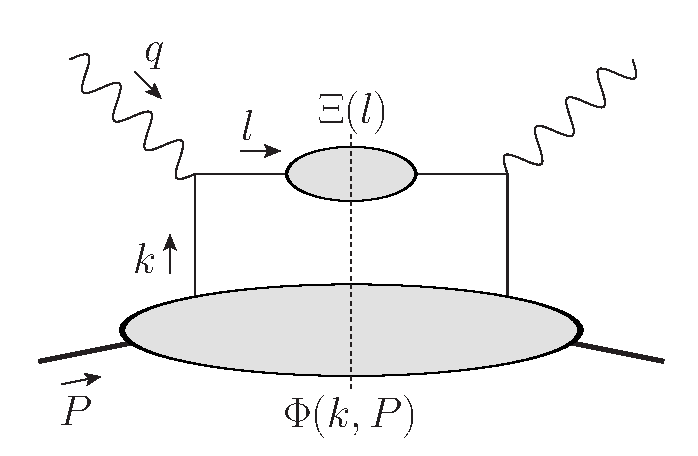
\includegraphics[width=0.3\linewidth,valign=t]{jetdiagram0}
  \hfill
  (b)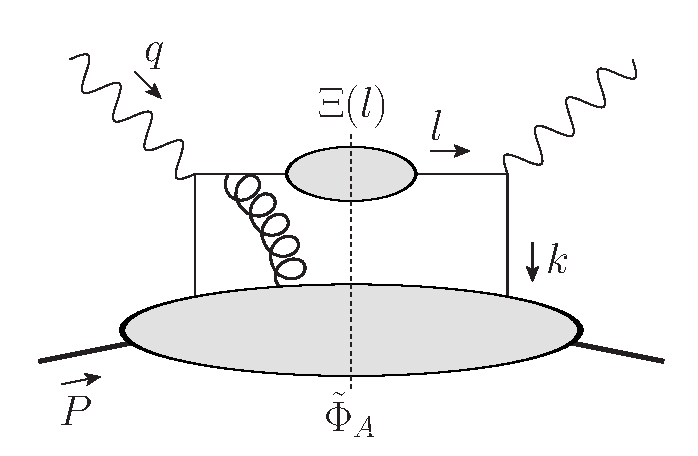
\includegraphics[width=0.3\linewidth,valign=t]{jetdiagram2}
  \hfill
  (c)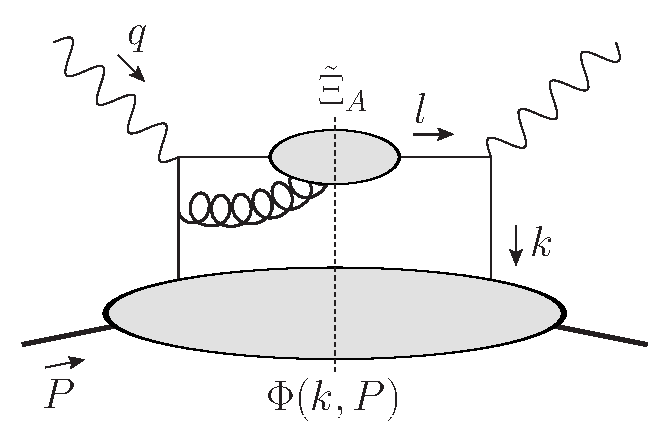
\includegraphics[width=0.3\linewidth,valign=t]{jetdiagram1}
  \caption{Diagrams contributing to DIS scattering up to twist-3 expansion, including a jet correlator in the top part. Note the gluon attaches to both the nucleon and jet correlators. The Hermitian conjugates of diagrams (b) and (c), i.e., with gluons attaching to the right of the cut, are not shown.
  }
  \label{fig:handbags}
\end{figure*}

When inserting the jet correlator in the handbag diagram for inclusive DIS, the invariant jet mass $\mu^2$ is integrated from 0 to $Q^2(1/x_B-1)$. This induces (kinematical) corrections of order $O(1/Q^2)$, whose effect on the $F_2$ structure function has been studied in Ref.~\cite{Accardi:2008ne}:
\begin{align}
  F_2(x_B) & = \int_0^{Q^2(1/x_B-1)}d\mu^2\, J_2(\mu^2) F_2^{(0)}(x_B(1+\mu^2/Q^2)) \ ,
\label{eq:F2}
\end{align}
where $F_2^{(0)}$ is the structure function calculated with the handbag
diagram sporting a bare quark propagator instead of the jet correlator, and
$\xi=2x_B/(1+\sqrt{1+4x_B^2M^2/Q^2})$ with $M$ the nucleon's mass is the
Nachtmann scaling variable. (We also omitted the dependence of the structure
function on $Q^2$ for clarity of notation). In this paper we limit our
attention to effects of order $O(1/Q)$ and therefore can extend the
integration to $\mu^2=\infty$. Therefore, the jet function $J_2$ decouples
and, thanks to the sum rule \eqref{eq:jetfnsprops}, integrates to 1. One then
recovers the conventional result, 
\begin{align}
  F_2(x_B) = \Big[ \int_0^\infty d\mu^2\, J_2(\mu^2) \Big] F_2^{(0)}(x_B) 
     + O(\Lambda^2/Q^2) = F_2^{(0)}(x_B)  + O(\Lambda^2/Q^2) \ .
\end{align}
%The same holds true also for the helicity structure function $g_1$.
%
More in general, the jet correlator decouples from the parton correlator $\Phi$ in any inclusive cross section calculation up to $O(1/Q)$, and the inclusive structure functions only depend on the integrated jet correlator 
\begin{equation} 
  \Xi(l^-) \equiv \int \frac{dl^2}{2l^-} d^2 l_T \, \Xi(l) 
    =  \frac{\Lambda}{2 l^-}\,\xi_1 {\bm 1}
    +  \xi_2 \frac{\nslash_-}{2} 
    + \text{higher\ twists}
    % +\frac{\Lambda^2}{4 (l^-)^2}\,\xi_3 \nslash_+
    % + i \frac{\Lambda}{2 l^-} \xi_4 
    % \frac{ \bigl[\nslash_-, \nslash_+ \bigr]}{2}.
\end{equation} 
where 
\begin{align}
\xi_1 &= \int d\mu^2 \frac{\mu}{\Lambda} J_1(\mu^2) 
       \equiv \frac{\mj}{\Lambda},
&
\xi_2 &= \int d\mu^2 J_2(\mu^2) = 1 \ .
% \\
% \xi_3 &= 0,
% &
% \xi_4 &= \int d\mu^2 \frac{\mu^2}{\Lambda^2} J_1(\mu^2) = \frac{\mjs}{\Lambda^2}.
\end{align} 
where $\mj$ can be interpreted as the average invariant mass produced in the spin-flip fragmentation processes of a quark of flavor $q$.
% The $\xi_1$ and $\xi_4$ have an interpretation as average invariant mass (and mass squared) of the current jet, and $l^-=q^- + O(1/Q)$ is imposed by 4-momentum conservation at the hard scattering vertex. The $\xi^4$ term contributes at order $O(1/Q^2)$ and is no further considered in this paper. 
It is important to notice that $\xi_2=1$ exactly due to CPT invariance \cite{Weinberg-book}, while $0 < \mj < \int d\mu^2 \mu J_2(\mu^2)$ is dynamically determined. From the analytic properties of spectral functions we may expect \cite{Accardi:2008ne)} $J_2(\mu^2) = Z \delta(\mu^2-m_q) + \bar J_2 (\mu^2) \theta (\mu^2-m_\pi^2)$ with the continuum starting at $m_\pi$, the mass of the pion, due to color confinement effects. Taking into account that $J_1 < J_2$, we may therefore expect 
\begin{align}
  \label{eq:mjet}
  \mj = O(10-100 \text{ MeV}) \ .
\end{align}
Although $\mj$ is in general a nonperturbative quantity, it is interesting to
notice that  
\begin{align}
  \label{eq:xi2_chiral_cond}
  \mj = \frac{\Lambda}{4} \int \Tr \big[ \Xi(l) \bm 1] 
   = \langle 0 | \bar \psi_i(0) \psi_i(0) | 0 \rangle
\end{align}
% \todo{[AA] 2 issues here: (1) possible factors of 4. 
% (2) I am neglecting the sum over quarks; we have to fix that somehow but there is a little tension between the quark level $\xi^a$ and the contribution to structure function which is summed and weighted by the electron charge.} 
Calculating this on the perturbative vacuum and limiting oneself to LO
corresponds to taking the trace of the cut bare-quark propagator to obtain 
$\mj = \,_{\text{pert}} \langle 0
|  \bar \psi_i(0) \psi_i(0) | 0 \rangle_{\text{pert}}  = \mq$, with $\mq$ the quark mass, recovering the
conventional result. However, we are here considering non perturbative effects
on the quark fragmentation and $\mj \gtrsim \mq$. 
%very importantly, this
%quantity can be computed in lattice QCD. 
%\todo{[AA] Are qe sure that $\mj > \mq$??}
%\todo{[AA] Need to discuss connection to quark condensate and tensor charge.}

\section{Twist-3 analysis}

Extending the analysis of \cite{Accardi:2008ne} to the calculation of twist-3
structure functions requires not only to consider the $\xi_1$ term in the jet
correlator, but also quark-gluon-quark correlators in both the proton and the
vacuum as depicted in Figs.\ref{fig:handbags}(b) and (c), respectively. 
In the former the $\xi_1$ terms contribute to $O(1/Q^2)$, so that up $O(1/Q)$
these give the same contribution as in the conventional handbag calculation.  

The novel element in our analysis is the jet's quark-gluon-quark correlator
$\Xi_A^{\mu}(l,k)$ in diagrams \ref{fig:handbags}(c), 
\begin{equation} 
\begin{split} 
  \left(\Xi_A^{\mu} \right)_{ij} &=
   \frac{1}{2}\, \sum_X \int \frac{\de \eta^+\, \de^2 \bm{\eta}_T}{(2\pi)^{3}}\;
   e^{\ii k \cdot \eta}\,
   \langle 0|\,
   {\cal U}^{n_+}_{(+\infty,\eta)}\,
   g A^{\mu}(\eta)\,
   \,\psi_i(\eta)|X\rangle
   \langle X|
             \bar{\psi}_j(0)\,
   {\cal U}^{n_+}_{(0,+\infty)}
   |0\rangle \bigg|_{\eta^-=0} .
\label{e:xi_A}
\end{split} 
\end{equation}  
This diagram and its hermitian conugate are not only important to account for all contribution of order $O(1/Q)$, but also in restoring up to twist-3 the gauge invariance broken in diagram \ref{fig:handbags}(a) by the different mass of the incoming and outgoing quark lines, namely, $\mq \neq \mj$.

Rather than directly using the definition \eqref{e:xi_A}, it is convenient to calculate the inclusive cross section as an integral of the semi-inclusive one, utilize the QCD equation of motions and furthermore summed over all hadron flavors, and take advantage of 
\begin{align}
  \label{eq:SIDIS_to_DIS}
  \sum_h \int \frac{d^3p_h}{(2\pi)2E_h} \Delta^h(l,p_h) = \Xi(l) \ , 
\end{align}
where $\Delta^h$ is the quark fragmentation correlator for production of a hadron of flavor $h$ and momentum $p_h$ \cite{New_testament}. In terms of the TMD fragmentation functions we are interested in, this reads
\begin{align}
  \label{eq:SIDIS_to_DIS_TMDlevel}
  \sum_h \int dz d^2p_{hT} z D_1^h(z,p_{hT}) & = \xi_2 = 1   \\
  \sum_h \int dz d^2p_{hT} E(z,p_{hT}) & = \xi_1 \ ,
\end{align}
where $D_1^h(z,p_{hT})$ is the twist-2 quark fragmentation function as a function of the hadron's collinear momentum fraction $z$ and transverse momentum $p_{hT}$, and $\tilde E^h(z,p_{hT})$ is a chiral-odd twist-3 function defined in \cite{New-testament}.

% As we shall see, an analogous formula for quark-gluon-quark correlators is not needed.
%The $\xi_1$ term is chiral-odd and therefore can appear in the inclusive cross section only coupled to the transversity function $h_1$. Therefore, for our analysis 
The relevant part of the semi-inclusive hadronic tensor for our analysis is 
\todo{[AA] I am using the notation in Piet Mulder's lecture notes - this will need to be checked.}
\begin{align}
  \label{eq:Wsidis_ini}
  2 \Lambda  W^{\mu\nu}
    & = i \frac{2\Lambda}{Q} \hat t^{[\mu}_{\phantom \perp} 
    \epsilon_\perp^{\nu]\rho}S_{\perp\rho} 
    \sum_q e_q^2
    \bigg[ 2 x_b g_T(x_B) \sum_h \int dz d^2p_{hT} D_1^{q,h}(z,p_{hT}) 
  %\\ &
  + 2 h_1(x_B) \sum_h \int dz d^2p_{hT} \tilde E^{q,h}(z,p_{hT}) \bigg] + \ldots
\end{align}
Here and we reintroduced the quark flavor $q$ for maximum clarity, and $e_q$ its electric charge.
The first term can be easily integrated with the help of the sum rule \eqref{eq:SIDIS_to_DIS_TMDlevel}. To integrate the latter, we first need make use of the relation $\tilde E(z) = E(z) - (\mq/\Lambda) z D_1(z)$, which is a consequence of the QCD equations of motion \cite{New-testament}, then utilize the sum rule \eqref{eq:SIDIS_to_DIS}:
\begin{align}
  \sum_h \int dz d^2p_{hT} \tilde E^{q,h}(z,p_{hT}) 
    = \sum_h \int dz d^2p_{hT} \Big[ E^{q,h}(z,p_{hT}) - \frac{\mq}{\Lambda} z D_1^{q,h}(z,p_{hT}) \Big]
    = \xi_1 - \frac{\mq}{\Lambda} \xi_2 = \frac{\mj - \mq}{\Lambda} \ .
\end{align}
This formula is the single most important result of this paper, and provides a non perturbative generalization of the commonly used $\int\tilde E =0$ sum rule introduced in \cite{Jaffe-Ji}. Indeed, calculating the jet correlator
on the perturbative vacuum one would obtain, as already discussed, $\mj=\mq$
and the new term would vanish.

Finally, with suitable projections of the hadronic tensor, the inclusive cross section up to order $\Lambda/Q$ can be written as
\begin{align}
\frac{d\sigma}{d\xbj \, dy\, d\psi}
%&
=
\frac{2 \alpha^2}{\xbj y Q^2}\,
\frac{y^2}{2\,(1-\varepsilon)}\, 
\biggl\{
&F_{UU ,T} + \varepsilon F_{UU ,L}
+ S_\parallel \lambda_e\,
  \sqrt{1-\varepsilon^2}\; 
F_{LL}
%\nonumber 
%\\  &
+ |\bm{S}_\perp| \lambda_e\, \sqrt{2\,\varepsilon (1-\varepsilon)}\, 
  \cos\phi_S\, 
F_{LT}^{\cos \phi_S}
 \biggr\} \ ,
\label{e:crossdis}
\end{align}
where the structure functions on the right hand side are defined as
\begin{align}
F_{UU ,T} &= \xbj\,\sum_q e_q^2\,f_1^q(\xbj),
\\
F_{UU ,L} &= 0,
\\
F_{LL} &=\xbj\,\sum_q e_q^2\,g_1^q(\xbj),
\\
F_{UT}^{\sin \phi_S}&=0,
\label{e:FUTint}
\\
F_{LT}^{\cos \phi_S}&=-\xbj\,\sum_q e_q^2\, \frac{2\Lambda}{Q}\,
\biggl(\xbj  g_T^q(\xbj)
   + \frac{\mj -\mq}{\Lambda} \, h_{1}^q(\xbj) \biggr).
\label{e:FLTint}
\end{align}
The second term in the last structure function is a new result from our
analysis; it is not suppressed as an inverse power of $Q$, and therefore
survives even in the Bjorken limit. On the non-perturbative
vacuum the jet mass is larger than the quark's, and this contributes a
non-negligible term to the twist-3 part of the $g_2$ function, as we will
discuss in the next section.  

 

\section{The $g_2$ structure function}

The new term in Eq.\eqref{e:FLTint} only appears in the $g_2$ structure function. Following the derivation in Ref.~\cite{ABMS}, one finds
\begin{align}
\label{e:g2}
  g_2(x_B) = g_2^{WW} + \frac{1}{2}\,\sum_a e_a^2
\biggl(
    \widetilde g_T^{a \star}(x) 
    + \int_x^1\frac{dy}{y} \widehat{g}_T^q(y) 
    + \frac{\mq}{\Lambda} \left(\frac{h_1^q}{x}\right)^\star(x) 
    + \frac{\mj-\mq}{\Lambda} \frac{h_1^q(x)}{x} 
\Biggr) \ ,
\end{align}
where we defined $f^*(x) = -f(x) + \int_x^1\frac{dy}{y} f(y)$. The first 4
terms coincide with the result obtained in the conventional handbag
approximation \cite{ABMS}, while the fifth is new. 

The first term is also known as the Wandzura-Wilczeck function $g_2^{WW} =
g_1^*(x)$ , and contains all the ``pure twist-2'' chiral even contributions to
the $g_2$ structure coming from quark-quark correlators. The second and third
terms contain all ``pure twist-3'' contributions, i.e., those coming from
quark-gluon-quark correlators. The fourth and fifth terms depend on the
transversity parton distribution function, $h_1$. 
The former is usually neglected for
light quarks since it is proportional to $\mq=O$(1 MeV). In the latter term,
new in our analysis, the transversity distribution is multiplied by a constant
of $O$(100 MeV), and cannot be a priori neglected.

It is important to estimate the size of teh variou scontributions to the non Wandzura-Wilczek part of $g_2$. We define the shorthand notation
\begin{align}
g_2^{tw3} & = \frac{1}{2}\,\sum_a e_a^2
    \biggl(
    \widetilde g_T^{a \star}(x) 
    + \int_x^1\frac{dy}{y} \widehat{g}_T^q(y) 
    \biggr) 
&
g_2^{\text{quark}} &= \frac{1}{2}\,\sum_a e_a^2 
 \frac{\mq}{\Lambda} (h_1^q/x)^\star(x),
&
g_2^{\text{jet}} &= \frac{1}{2}\,\sum_a e_a^2 
\frac{\mj-\mq}{\Lambda} \frac{h_1^q(x)}{x}. 
\end{align} 
These are comapred in Figure~\ref{f:g2contrib} to the $g_2-g_2^{WW}$ function obtained in the very recent JAM15 fit of polarized DIS asymmetries \cite{JAM15}, that includes a large amount of precise data at large $x$ from Jefferson Lab, and simultaneously fits the higher-twist components of in $g_1$ and $g_2$ to the data. For the ``pure twist-3'' contribution, $g_2^{tw3}$, {\it i.e.}, the contribution from quark-gluon-quark matrix elements, we show a model calculation by Braun et al. \cite{Braun-et-al}; for other estimates, see \cite{Other-tw3-calcs}. To estimate the contributions from quark ($g_2^q$) and jet mass ($g_2^{jet}$) effects, that depend on chiral odd quark-quark matrix elements, we use the recent Pavia15 fit of the transversity distribution from Ref.~\cite{Radici:2015mwa}, which is comparable also to other
extractions~\cite{Anselmino:2013vqa,Kang:2015msa}. Furthermore, we choose the values of the mass parameters to be $\mq=5$ MeV and $\mj = 100$ MeV.

As one can see, in the proton case the pure twist-3 contribution is quite smaller in magnitude, and opposite in sign, compared to the JAM15 fit. As expected, the quark-mass contribution is essentially negligible and cannot reconcile these two. Even though the uncertainties in the $h_1$ extraction and even more the estimate of $M_q$ are large, it is quite clear that the gap between the pure twist-3 $g_2^{tw3}$ function and the JAM15 fit can be explained by the new jet-mass contribution we discussed in this paper. 

In the neutron case, the jet contribution is very negative at intermediate to large values of $x$. If one trusts the order of magnituse of the $g_2^{tw3}$ calculation by Braun et al., one would conclude that the jet contribution cannot be that large. However, the latteris dominated by the $d$ quark's transversity, whose fit suffers from large systematic uncertainties and saturates the negative Soffer bound.Recent deata in $p+p$ collisions indicate, however, that $h_1^d$ is less negative than in the Pavia15 fits, in agreement with the JAM15 fit of the non Wandzura-Wilczek contribution to $g_2$. Correspondingly the jet contribution to the proton at $x \approx 0.1$ would become less positive, inproving as well teh agreement with the JAM15 fit.


\begin{itemize}
\item smaller-$x$: constrains the small-$x$ behavior of transversity.
\end{itemize}
Some ideas to check:
\begin{itemize}
\item JAM13 neutron has almost 0 twist 3, with small positive contribution at small x. Can we use this to highlight teh $g_2^{jet}$ contribution? Or maybe as a cnstrain: if Braun is right then $g_2^{jet}(n) \approx -g_2^{tw3}(n)$. (still, does not help much for the proton).
\item In Jam 13, Fig. 6, it looks like in general the violation of teh BC sum rule is a small-x effect --> constraints on h(x) fits? This cannot really be checked vs. JAM15, that assumes $g_2^(0)$ respects BC. 
\end{itemize}

\begin{figure}[tbh]
\begin{center}
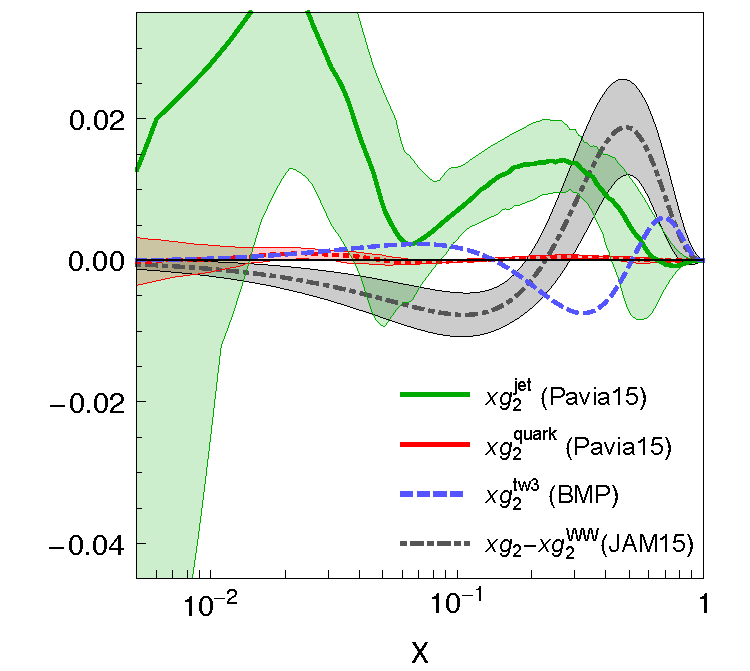
\includegraphics[width=8cm]{g2contrib}
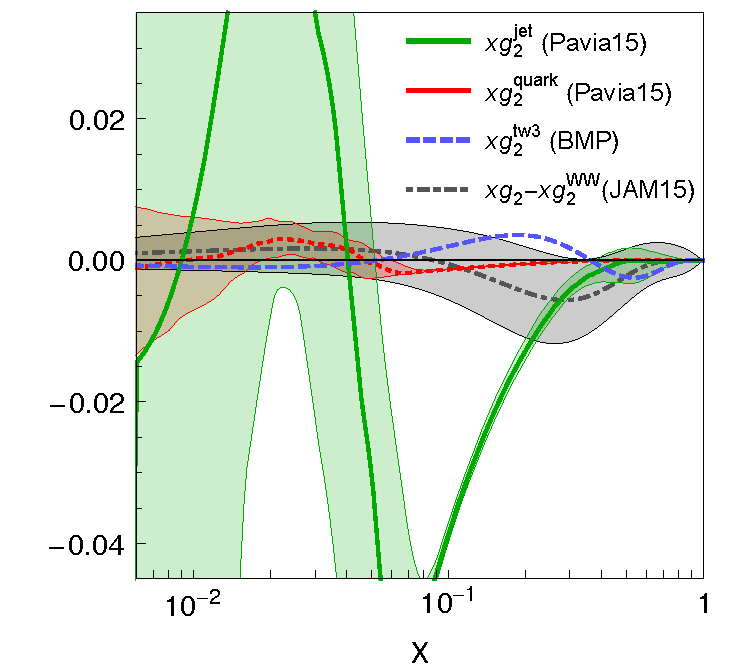
\includegraphics[width=8cm]{g2contribN}
\caption{\label{f:g2contrib} 
Different contributions to the non Wandzura-Wilczek part of the proton (left) and neutron (right) $g_2$ structure function compared to the JAM15 fit of the  $g_2-g_2^{\text{WW}}$ (solid black) \cite{JAM15}. The quark and jet contributions are shown with a dotted red and a dot-dashed green line respectively, with uncertainty bands coming form the Pavia15 fit of the transversity function \cite{Pavia15}. The unceratainty in the choice $m_q=5$ GeV and $M_q=100$ GeV is not shown. The pure twist-3 contribution calculated by Braun et al. \cite{Braun-et-al} is shown as a dashed blue line (no uncertainty estiamte was provided in teh original reference).
}
\end{center}
\end{figure}

It is interesting to consider the moments of the non Wandzura-Wilczek contribution to $g-2$,
\begin{align}
  d_N = N \int_0^1 x^N \big( g_2(x) - g_2^{WW}(x) \big) \ .
\end{align}
For a generic function $f$, let us define it's $N$-th moment as $f[N]=\int_0^1 dx\, x^{N-1} f(x)$. It is then straightforward to verify that $f^*[N] = f[N] (N-1)/N$ and  
\begin{align}
  d_N & \equiv N g_2[N+1] + (N-1) g_1[N+1] \\
  & = \frac12 \sum_q e_q^2 \bigg( N \tilde g_T^q[N+1] + \hat g_T^q[N+1]
    + \frac{N M_q-m_q}{\Lambda} h_1^q[N+1] \bigg) \ .
\end{align}
\AAcom{The notation used in JAM15 with $x^{N-1}$ for the Nth moment is pretty awkward here. Should we use $x^N$ instead?}

The zero-th moment corresponds to an extension of teh Burkhardt-Cottingham sum rule \cite{BC,Jaffe-lectures}, that appears to be broken by the non-perturbative spin-flip contribution from the jet function: 
\begin{align}
  \label{eq:BC}
  \int dx\, g_2(x) = \frac{\mj-\mq}{\Lambda} \int dx\, \frac{1}{x} h_1(x) \ .
\end{align}
This sum rule, in which the pure twist-3 part does not take part, is a consequence of the Lorentz invariance of the DIS cross section, that entails $\int_0^1 dx g_1^a(x) = \int_0^1 g_T^q(x)$. It explicitly displays a contribution from spin-flip processes, that are included in the original derivation by Burkhardt and Cottingham \cite{BC} but do not show up in treatments that only consider free field quark propagators for the struck quark \cite{Jaffe-lectures}. 

Assuming the Burkhardt-Cottingham sum rule to be strictly valid, we obtain a strong constraint on the transversity function,
\begin{align}
   \int dx\, \frac{1}{x} h_1(x) = 0 \ .
\end{align}
Even if the BC sun rule is broken by a 
$J = 0$ fixed pole with non-polynomial residue, i.e., if $g_2$ integrates to a finite but non-zero number \cite{Jaffe-lectures}), we obtain that $h_1(x)/x$ must be integrable. This entails a bound on the small $x$ behavior of the transversity,
\begin{align}
  h_1(x) \propto x^\epsilon \ \ \ \epsilon>0 \ .
\end{align}
This bound will be very useful, \eg, in transversity fits, where the data at small $x$ is as yet very limited.


{\bf [---------------- AA:  EDITED down here --------------------]}



Consequences:
\begin{itemize}
\item Inclusive DIS become sensitive to the tensor charge; furthermore, teh BC summ rule isolates the effects due to the chiral odd part of the jet correlator. 
\item Both the jet mass $\mj$ and the tensor charge can in principle be calculated on the lattice
\item Comparison to the Burkhardt-Cottingham sum rule can provide experimental verification of lattice calculation
\item in turn these can be used to determine the size of the $h_1$ term in $g_2-g_2^{WW}$ and allow an eperimental extraction of the pure twist-3 terms.
\item Recent calcs of $g_T^{d-u}$ tensor charge are very precise - can we use this info in our plots? (to ``measure'' the quark condenstae $\langle0|\psi\bar\psi|0\rangle>$, for example? this would need an estimate of teh BC breaking, that is only availbal efrom JAM13, for all that I know.)
\end{itemize}

It is important to explore in which other process does $\mj$ contribute, as to provide an experimental check of the formalism:
\begin{itemize}
\item inclusive $\Lambda$ production in $e^+ + e^-$
\item same-side dihadrons in $e^+ + e^-$ 
\end{itemize}
\todo{It would be cool to find a process where the $\mj$ contribution is th eonly one (similar to the BC breaking) ...}   



%%%%%%%%%%%%%%%%%%%%%%%%%%%%%%%%%%%%%%%%%%%%%%%%%%%%%%%%%%%%%%%%%%%%%%%%%
\section{Conclusions}


%%%%%%%%%%%%%%%%%%%%%%%%%%%%%%%%%%%%%%%%
%%%%%%%%% ACKNOWLEDGMENTS %%%%%%%%%%%%%%
%%%%%%%%%%%%%%%%%%%%%%%%%%%%%%%%%%%%%%%%

\begin{acknowledgments}
This work was supported by DOE contract No. DE-AC05-06OR23177,
under which Jefferson Science Associates, LLC operates Jefferson Lab, by the DOE contract DE-SC008791 and 
by the European Research Council (ERC) under the European Union's 
Horizon 2020 research and innovation programme (grant agreement No. 647981,
3DSPIN)
\end{acknowledgments}


\bibliographystyle{myrevtex}
\bibliography{mybiblio}

\end{document}
